\section*{Questão 2}

\subsection*{Definição da Cadeia de Markov}

A cadeia de Markov para este problema é definida pelos seguintes elementos:

\begin{enumerate}
    \item \textbf{Estados}: Representados pela tupla $(c, s)$, onde:
    \begin{itemize}
        \item $c$ é o número de clientes no sistema (limitado entre 0 e 8).
        \item $s$ é o número de servidores disponíveis (limitado entre 1 e 3).
    \end{itemize}

    \item \textbf{Ações}: As ações disponíveis em cada estado são:
    \begin{itemize}
        \item $-1$: Remover um servidor.
        \item $0$: Manter o número atual de servidores.
        \item $+1$: Adicionar um servidor (respeitando os limites).
    \end{itemize}

    \item \textbf{Transições}: Determinadas pelas probabilidades de chegada de novos clientes no final de cada intervalo de tempo:
    \begin{itemize}
        \item $p_0 = 0.4$: Probabilidade de 0 clientes chegarem.
        \item $p_2 = 0.2$: Probabilidade de 2 clientes chegarem.
        \item $p_4 = 0.4$: Probabilidade de 4 clientes chegarem.
    \end{itemize}
    A transição entre estados considera:
    \begin{itemize}
        \item Atendimento: $\min(c, s)$ clientes são atendidos no início de cada intervalo.
        \item Clientes restantes: Permanecem no sistema para o próximo intervalo.
        \item Restrições: O número total de clientes no sistema é limitado a 8.
    \end{itemize}

    \item \textbf{Ordem dos eventos}: Para cada intervalo de tempo, a ordem dos eventos considerada é:
    \begin{enumerate}[label=\roman*.]
        \item Atendimento de clientes.
        \item Adição/remoção de servidores.
        \item Chegada de clientes.
    \end{enumerate}

    \item \textbf{Recompensas}: A recompensa para cada transição é composta por:
    \begin{itemize}
        \item Ganho por cliente atendido: $T \cdot \min(c, s)$, com $T = 10$.
        \item Custo por servidor: $-R_s \cdot s'$, com $R_s = 5$.
        \item Penalidade por fila: $-R_q$ se $c' > 4$, caso contrário $0$, com $R_q = 10$.
        \item Penalidade por ociosidade: $-R_0$ por servidor não utilizado, max($s' - c', 0$), com $R_0 = 2$.
    \end{itemize}
    Onde $c$ e $s$ são os valores de clientes e servidores no estado atual e $c'$ e $s'$ são os valores no próximo estado.
\end{enumerate}

\subsection*{Solução por \textit{Value Iteration}}

Foi implemmentado em Python uma função que calcula a política ótima para a cadeia de Markov descrita. O código fonte está disponível no repositório indicado no final deste relatório, na pasta \texttt{lista\_6}, arquivo \texttt{value\_itaration.py}. O código principal, onde são definidas as probabilidades de transição e as recompensas, está disponível no arquivo \texttt{main.py}. O código segue o seguinte fluxo:

\begin{enumerate}
    \item Inicializa \( V[s] = 0 \) para todos os estados \( s \).
    \item Iterativamente calcula os valores \( V[s] \) para cada estado, atualizando-os com base na equação de Bellman:
    \[
    V(s) = \max_a \sum_{s', r} P(s', r \mid s, a) \cdot \left( r + \gamma \cdot V(s') \right).
    \]
    \item Em cada iteração, verifica a convergência comparando a maior mudança (\( \Delta \)) entre os valores antigos e novos. O loop termina quando \( \Delta < \theta \), o limiar definido.
    \item Após convergir, calcula a política ótima \( \pi^*(s) \) para cada estado, escolhendo a ação \( a \) que maximiza o valor esperado \( V(s) \):
    \[
    \pi^*(s) = \arg\max_a \sum_{s', r} P(s', r \mid s, a) \cdot \left( r + \gamma \cdot V(s') \right).
    \]
    \item Retorna a função de valor ótima \( V(s) \) e a política ótima \( \pi^*(s) \).
\end{enumerate}

Foi utilizado um fator de desconto $\gamma = 0.9$ e um limiar de convergência $\theta = 1e-6$. Para esses valores, a convergência ocorreu em 2457 iterações. A função de valor ótima calculada e a política ótima derivada dela são apresentadas na figura \ref{fig:value_iteration_policy_and_values}.
A variação de $\Delta$ ao longo das iterações é apresentada na figura \ref{fig:value_iteration_delta}.

\begin{figure}[H]
    \centering
    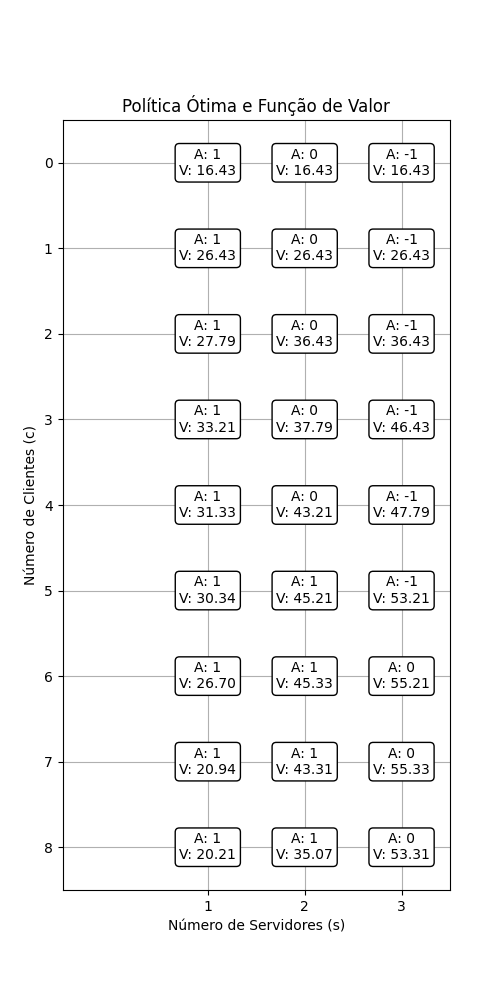
\includegraphics[width=0.5\textwidth]{fig/value_iteration_policy_and_values.png}
    \caption{Função de valor ótima e política ótima calculadas por \textit{Value Iteration}.}
    \label{fig:value_iteration_policy_and_values}
\end{figure}

\begin{figure}[H]
    \centering
    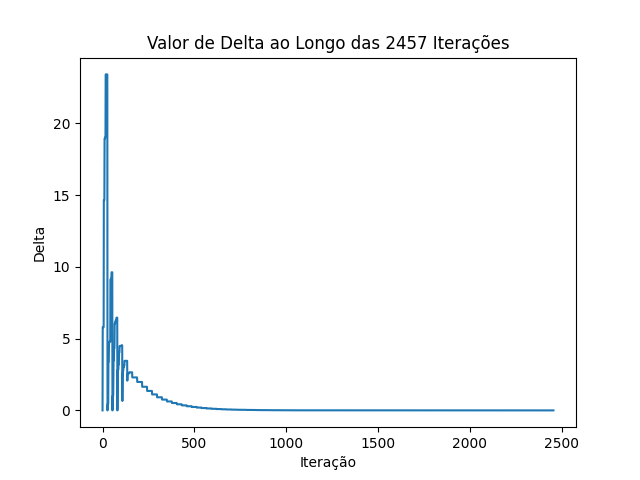
\includegraphics[width=0.5\textwidth]{fig/value_iteration_delta.png}
    \caption{Variação de $\Delta$ ao longo das iterações de \textit{Value Iteration}.}
    \label{fig:value_iteration_delta}
\end{figure}



\subsection*{Solução por \textit{Policy Iteration}}

Foi implementado em Python uma função que calcula a política ótima para a cadeia de Markov descrita. O código fonte está disponível no repositório indicado no final deste relatório, na pasta \texttt{lista\_6}, arquivo \texttt{policy\_itaration.py}. O código principal, onde são definidas as probabilidades de transição e as recompensas, está disponível no arquivo \texttt{main.py}. O código segue o seguinte fluxo:

\begin{enumerate}
    \item Inicializa uma política arbitrária \( \pi(s) = -1 \) e uma função de valor \( V(s) = 0 \) para todos os estados \( s \).
    \item \textbf{Etapa 1 - Avaliação da Política:}
    \begin{enumerate}
        \item Para cada estado \( s \), atualiza \( V(s) \) usando a equação:
        \[
        V(s) = \sum_{s',r} P(s', r \mid s, \pi(s)) \cdot \left( r + \gamma \cdot V(s') \right).
        \]
        \item Repete as atualizações até que a maior mudança em \( V(s) \) entre duas iterações seja menor que um limiar \( \theta \).
    \end{enumerate}
    \item \textbf{Etapa 2 - Melhoria da Política:}
    \begin{enumerate}
        \item Para cada estado \( s \), identifica a melhor ação \( a \) que maximiza o valor esperado:
        \[
        \pi(s) = \arg\max_a \sum_{s', r} P(s', r \mid s, a) \cdot \left( r + \gamma \cdot V(s') \right).
        \]
        \item Se a nova política \( \pi(s) \) for igual à política anterior para todos os estados, o algoritmo termina. Caso contrário, retorna à etapa de avaliação.
    \end{enumerate}
    \item Retorna a política ótima \( \pi^*(s) \) e a função de valor ótima \( V^*(s) \).
\end{enumerate}

Foi utilizado um fator de desconto $\gamma = 0.9$ e um limiar de convergência $\theta = 1e-6$. Para esses valores, a convergência ocorreu em 4 iterações do laço externo \textit{while principal}, porém foram contabiizadas um total de 5292 iterações internas da etapa de avaliação da política. A função de valor ótima calculada e a política ótima derivada dela são apresentadas na figura \ref{fig:policy_iteration_policy_and_values}. A variação de $\Delta$ ao longo das iterações é apresentada na figura \ref{fig:policy_iteration_delta}.

\begin{figure}[H]
    \centering
    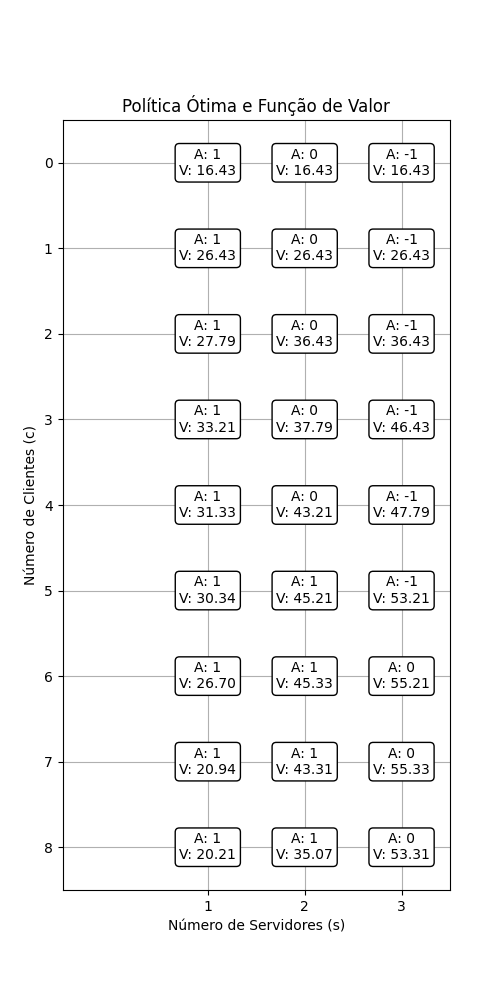
\includegraphics[width=0.5\textwidth]{fig/policy_iteration_policy_and_values.png}
    \caption{Função de valor ótima e política ótima calculadas por \textit{Policy Iteration}.}
    \label{fig:policy_iteration_policy_and_values}
\end{figure}

\begin{figure}[H]
    \centering
    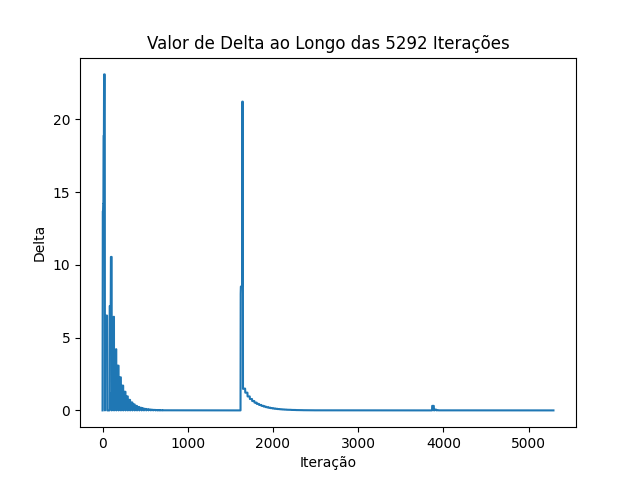
\includegraphics[width=0.5\textwidth]{fig/policy_iteration_delta.png}
    \caption{Variação de $\Delta$ ao longo das iterações de \textit{Policy Iteration}.}
    \label{fig:policy_iteration_delta}
\end{figure}

\subsection*{Q-Learning}

Foi implementado em Python um algoritmo de \textit{Q-Learning} para resolver o problema da cadeia de Markov descrita. O código fonte está disponível no repositório indicado no final deste relatório, na pasta \texttt{lista\_6}, arquivo \texttt{q\_learning.py}. O código principal, onde são definidas as probabilidades de transição e as recompensas, está disponível no arquivo \texttt{main.py}. Como o problema em questão não possui estado terminal, o algoritmo foi adaptado para, a cada epsódio, limitar o número de passos. Além disso, foi implementada uma classe \texttt{EnvironmentSimulator} para simular o ambiente, recebendo como entrada o estado atual e a ação tomada e retornando o próximo estado e a recompensa obtida. A classe \texttt{EnvironmentSimulator} encontra-se no arquivo \texttt{utils.py}. O código do lgoritmo de \textit{Q-Learning} segue o seguinte fluxo:

\begin{enumerate}
    \item Inicializa \( Q(s, a) \) com zeros para todos os estados e ações.
    \item Para cada episódio:
    \begin{enumerate}
        \item Escolhe um estado inicial aleatório.
        \item Para cada passo no episódio:
        \begin{enumerate}
            \item Escolhe uma ação (usando política \( \epsilon \)-gulosa):
            \begin{itemize}
                \item Com probabilidade \( \epsilon \), escolhe uma ação aleatória (\textit{exploration}).
                \item Caso contrário, escolhe a ação que maximiza \( Q(s, a) \) (\textit{exploitation}).
            \end{itemize}
            \item Simula o ambiente com a ação escolhida para obter:
            \begin{itemize}
                \item O próximo estado \( s' \).
                \item A recompensa \( r \).
            \end{itemize}
            \item Atualiza \( Q(s, a) \) usando a equação de aprendizado por diferença temporal (TD):
            \[
            Q(s, a) \leftarrow Q(s, a) + \alpha \left[ r + \gamma \max_{a'} Q(s', a') - Q(s, a) \right]
            \]
            \item Atualiza o estado atual para \( s' \).
            \item Se atingir o número máximo de passos, termina o episódio.
        \end{enumerate}
        \item Após o episódio, calcula:
        \begin{itemize}
            \item A nova função de valor \( V(s) = \max_a Q(s, a) \).
            \item A mudança absoluta máxima \( \Delta V = \max_s |V_{\text{novo}}(s) - V(s)| \).
        \end{itemize}
        \item Atualiza \( V(s) \) e armazena \( \Delta V \) para análise de convergência.
    \end{enumerate}
    \item Deriva a política ótima \( \pi^*(s) \) escolhendo, para cada estado, a ação que maximiza \( Q(s, a) \).
    \item Retorna a política ótima \( \pi^*(s) \), a função de valor \( V(s) \), e a lista de \( \Delta V \) ao longo dos episódios.
\end{enumerate}

Foram utilizados os seguintes hiperparâmetros: fator de desconto \( \gamma = 0.9 \), taxa de aprendizado \( \alpha = 0.1 \), probabilidade de exploração \( \epsilon = 0.1 \), número de episódios \( 1000 \) e limite de passos por episódio \( 100 \). Como não há um critério de convergência, o algoritmo executa 100 mil iterações. A função de valor ótima calculada e a política ótima derivada dela são apresentadas na figura \ref{fig:q_learning_policy_and_values}. A variação de \( \Delta V \) ao longo dos episódios é apresentada na figura \ref{fig:q_learning_delta}.

\begin{figure}[H]
    \centering
    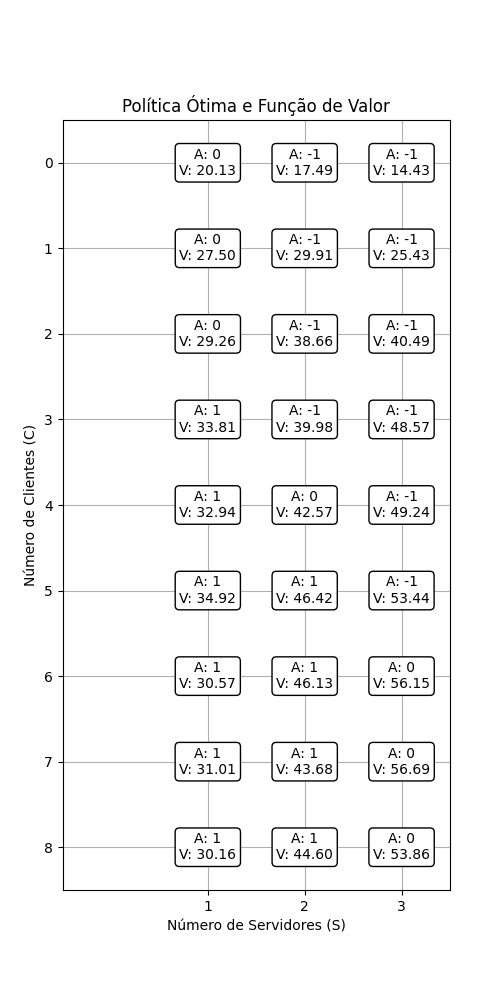
\includegraphics[width=0.5\textwidth]{fig/q_learning_policy_and_values.png}
    \caption{Função de valor ótima e política ótima calculadas por \textit{Q-Learning}.}
    \label{fig:q_learning_policy_and_values}
\end{figure}

\begin{figure}[H]
    \centering
    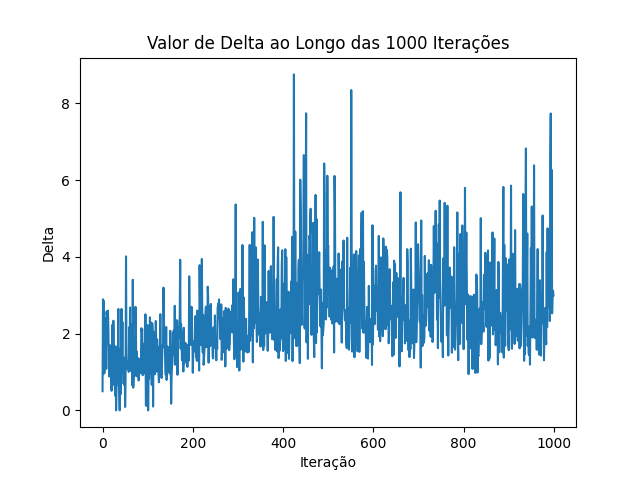
\includegraphics[width=0.5\textwidth]{fig/q_learning_delta.png}
    \caption{Variação de \( \Delta V \) ao longo dos episódios de \textit{Q-Learning}.}
    \label{fig:q_learning_delta}
\end{figure}

OBS: devido a aleatoriedade do algoritmo, e a falta de um estado terminal, não é possível observar uma convergência clara na figura \ref{fig:q_learning_delta}, como nos métodos anteriores. Entretanto é possível observar que os valores de \( V^* (s) \) para cada estado na figura \ref{fig:q_learning_policy_and_values} são próximos dos valores obtidos pelos métodos anteriores e as ações da política ótima também são semelhantes. Foram feitas várias execuções do algoritmo alterando os hiperparâmetros, e nenuma delas fez ele convergir.

\subsection*{Comparação dos Métodos}

Abaixo vemos as figuras \ref{fig:value_iteration_policy_and_values}, \ref{fig:policy_iteration_policy_and_values} e \ref{fig:q_learning_policy_and_values} exibidas lado a lado.

% plot das figuras usando subfigure
\begin{figure}[H]
    \centering
    \begin{subfigure}{0.3\textwidth}
        \centering
        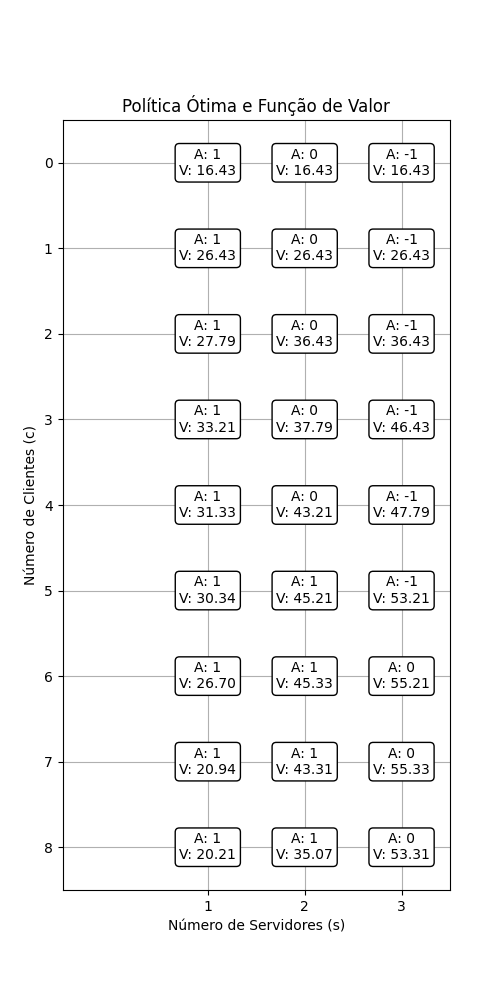
\includegraphics[width=\linewidth]{fig/value_iteration_policy_and_values.png}
        \caption{\textit{Value Iteration}}
    \end{subfigure}
    \begin{subfigure}{0.3\textwidth}
        \centering
        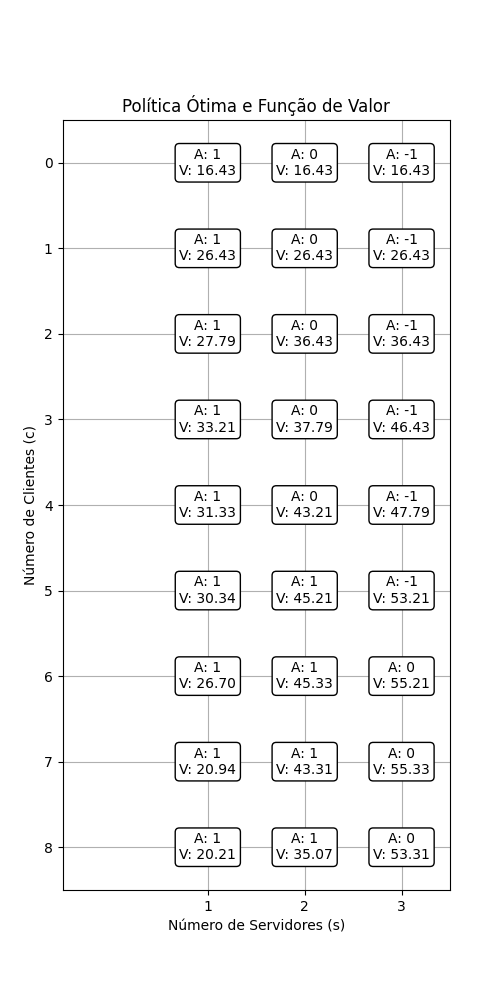
\includegraphics[width=\linewidth]{fig/policy_iteration_policy_and_values.png}
        \caption{\textit{Policy Iteration}}
    \end{subfigure}
    \begin{subfigure}{0.3\textwidth}
        \centering
        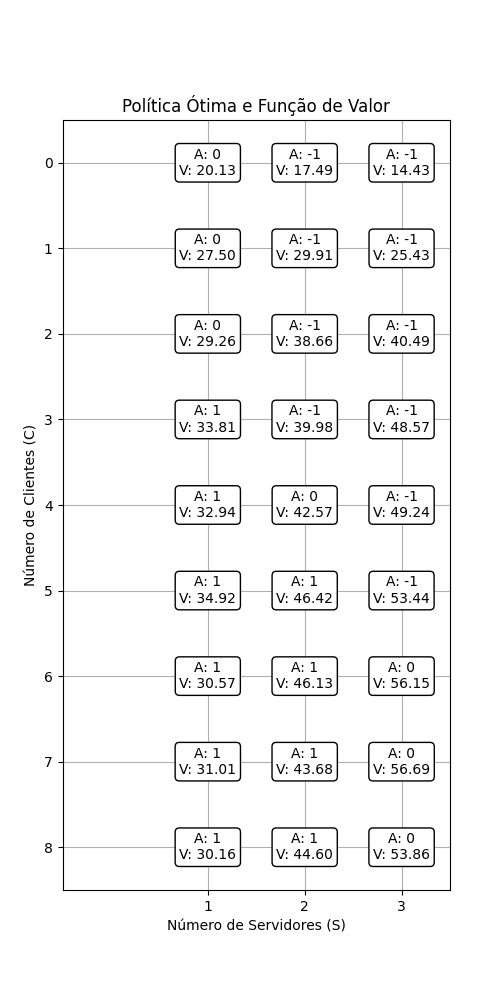
\includegraphics[width=\linewidth]{fig/q_learning_policy_and_values.png}
        \caption{\textit{Q-Learning}}
    \end{subfigure}
    \caption{Comparação das políticas e funções de valor ótimas calculadas pelos métodos.}
    \label{fig:comparison}
\end{figure}

O métodos \textit{Value Iteration} e \textit{Policy Iteration} apresentaram resultados identicos, com mesma política ótima e função de valor ótima. O método \textit{Q-Learning} apresentou resultados semelhantes, com valores de \( V^* (s) \) próximos e ações semelhantes a da política ótima. Entretanto, o método \textit{Q-Learning} não convergiu, possivelmente devido a aleatoriedade do algoritmo e a falta de um estado terminal.

O método \textit{Value Iteration} foi o mais rápido, convergindo em 2457 iterações. O método \textit{Policy Iteration} foi o segundo mais rápido, convergindo em 4 iterações do laço externo \textit{while principal}, porém foram contabiizadas um total de 5292 iterações internas da etapa de avaliação da política. O método \textit{Q-Learning}, por não ter um critério de convergência, executando sempre o mesmo número de passos vezes o número de episódios, foi o mais lento, com 100 mil iterações.


